% options:
% thesis=B bachelor's thesis
% thesis=M master's thesis
% czech thesis in Czech language
% slovak thesis in Slovak language
% english thesis in English language
% hidelinks remove colour boxes around hyperlinks

\documentclass[thesis=M,czech]{FITthesis}[2012/06/26]

\usepackage[utf8]{inputenc} % LaTeX source encoded as UTF-8

\usepackage{graphicx} %graphics files inclusion
% \usepackage{amsmath} %advanced maths
% \usepackage{amssymb} %additional math symbols

\usepackage{dirtree} %directory tree visualisation

% % list of acronyms
% \usepackage[acronym,nonumberlist,toc,numberedsection=autolabel]{glossaries}
% \iflanguage{czech}{\renewcommand*{\acronymname}{Seznam pou{\v z}it{\' y}ch zkratek}}{}
% \makeglossaries

\newcommand{\tg}{\mathop{\mathrm{tg}}} %cesky tangens
\newcommand{\cotg}{\mathop{\mathrm{cotg}}} %cesky cotangens

% % % % % % % % % % % % % % % % % % % % % % % % % % % % % % 
% ODTUD DAL VSE ZMENTE
% % % % % % % % % % % % % % % % % % % % % % % % % % % % % % 

\department{Katedra softwarového inženýrství}
\title{Children Usability Lab - management video streamů}
\authorGN{Patrik} %(křestní) jméno (jména) autora
\authorFN{Faistaver} %příjmení autora
\authorWithDegrees{Bc. Patrik Faistaver} %jméno autora včetně současných akademických titulů
\supervisor{Ing. Jiří Chludil}
\acknowledgements{Rád bych poděkoval vedoucímu mé diplomové práce Ing. Jiřímu Chludilovi i oponentovi Ing. Jiřímu Melnikovovi za užitečné připomínky a mnoho cenných rad. Dále chci poděkovat své rodině a blízkým přátelům za podporu a motivaci při tvorbě této práce i během celého studia.}
\abstractCS{Tato diplomová práce navazuje na bakalářskou práci Karolíny Solanské s názvem Children Usability Lab - aplikace pro správu laboratoře. Její bakalářská práce je zde rozšířena o návrh a implementaci subsystému pro management veškerých záznamů nahrávaných v laboratoři Children Usability Lab. Součástí této práce je také analýza současného systému i existujících řešení pro požadovanou správu záznamů, dále pak návrh, realizace a její následné testování. Implementované rozšíření stávajícího systému plně pokrývá dohodnuté zadání i specifikované požadavky.
\par
 Závěrem této diplomové práce je podrobení subsystému integračním i akceptačním testům. Subsystém se podařilo úspěšně nasadit do počítačového prostředí laboratoře Children Usability Lab, kde usnadňuje a zefektivňuje tamní usability testování.}

\abstractEN{Sem doplňte ekvivalent abstraktu Vaší práce v~angličtině.}
\placeForDeclarationOfAuthenticity{V~Praze}
\declarationOfAuthenticityOption{4} %volba Prohlášení (číslo 1-6)
\keywordsCS{testování použitelnosti, webová aplikace, laborator uživatelského testování, management záznamů, správa videa}
\keywordsEN{Nahraďte seznamem klíčových slov v angličtině oddělených čárkou.}

\begin{document}

% \newacronym{CVUT}{{\v C}VUT}{{\v C}esk{\' e} vysok{\' e} u{\v c}en{\' i} technick{\' e} v Praze}
% \newacronym{FIT}{FIT}{Fakulta informa{\v c}n{\' i}ch technologi{\' i}}

\begin{introduction}
Testování použitelnosti je proces při kterém se aplikace testuje přímo za pomocí vzorku koncových uživatelů a díky kterému 
se autoři aplikace dozvědí, jak jsou různé prvky uživatelského rozhraní srozumitelné a jak dobře jsou uživatelé schopni se v aplikaci orientovat. V současném světě technologií tento proces vyžaduje informační systém jako řešení pro usnadnění testování, plánování i komunikace mezi jednotlivými subjekty v laboratoři testování použitelnosti. Vývoj takovéhoto systému byl zahájen bakalářskou prací Karolíny Solanské s názvem Children Usability Lab - aplikace pro správu laboratoře (odkazem \cite{solankar}). Její práce vyvinula systém, který slouží jako webová aplikace zajišťující plánování a organizaci testů použitelnosti. Zmíněná předchozí bakalářská práce měla neobvykle větší počet stran a přesto je v implementovaném systému spoustu možností pro vyvinutí nových funkcí. Na tomto základě se dá říci, že se jedná o celkem rozsáhlý systém. Jeden ze směrů, kterým by se systém mohl začít rozšiřovat byla veškerá práce s videem což bylo ostatně zmíněno v kapitole o dalším vývoji.

Laboratoř použitelnosti na Fakultě informačních technologií ČVUT v Praze je vybavena spoustou zařízení, která jsou schopná zaznamenávat různorodá data. Jedná se nejen o všechna výpočetní zařízení, na kterých probíhají samotné testy, jako hlavní stolní počítač, tablet apod., ale také spousta kamer, mikrofonů či dokonce snímač pohybu očí po obrazovce. Není pochyb o tom, že data z těchto nahrávání schopných zařízení mohou značně přispět ke zkvalitnění vyhodnocování testů použitelnosti. V aktuálním stavu je práce se záznamy velice obtížná a neúčinná, jak je uvedeno v kapitole o současném stavu (). Z těchto důvodů je nutné rozšířit stávající systém o funkcionalitu, která práci s těmito záznamy značně ulehčí a zefektivní. Jedná se o to, aby uživatelé systému mohli jednoduše pouze přes webové rozhraní spustit a zastavit nahrávání z vybraných zařízení, záznamy roztřídit, uložit v požadovaném formátu a kompresi, upravovat zadaným výčtem způsobů, poslat přes síť do systému SAGE a podobně.


-------------------------
Testování použitelnosti samotné je pomerne složitý proces vyžadující ruzné
druhy dokumentace. Bezproblémový prubeh také vyžaduje dobrou komunikaci
mezi úcastníky testování, organizátory i zadávající firmou. Pro laborator
použitelnosti na FIT CVUT je tedy treba vytvorit systém, který by byl schopen
splnit tyto funkce a poskytl svým uživatelum všechny potrebné informace.
Vetšina lidí dnes používá internet alespon v nejaké míre a cílová skupina laboratore
na testování použitelnosti - tedy majitelé firem ci vývojári - se bez
nej v podstate neobejde.
Provoz laboratore použitelnosti vyžaduje velmi dobrou organizaci a použitelný
informacní systém se tedy jeví jako dobré rešení pro usnadnení testování, plánování
i komunikace mezi jednotlivými subjekty.
Jelikož se laborator na FIT CVUT zameruje na testování použitelnosti s detmi,
v práci se zároven zabývám specifikací, jak presne by melo probíhat testování
použitelnosti a jeho jednotlivé náležitosti a zároven jak tento proces prizpusobit
detským uživatelum.

\end{introduction}

\chapter{Cíl práce}

\chapter{Analýza}

\section{Definice pojmů} \label{sec:analyza_definice_pojmu}
\textbf{Frontend}\\
Jedná se o část aplikace, která je viditelná běžným uživatelům.\\ \\
\textbf{Backend}\\
Jedná se o část aplikace, uživatelům \uv{schovaná} za frontendem a slouží především ke zpracování dat.\\ \\

\section{Rozbor zadání} \label{sec:analyza_rozbor_zadani}
\begin{enumerate}
	\item \textbf{Analyzujte a aktualizujte funkční i nefunkční požadavky zaměřené na správu videa, uvedené v předchozí
práci.\\}
	Jak již bylo zmíněno, tak tato práce navazuje na bakalářskou práci Karolíny Solanské s názvem Children Usability Lab - aplikace pro správu laboratoře (odkazem \cite{solankar}). Aby navázání na předchozí práci mělo ten správný směr, je nutné analyzovat specifické požadavky z předchozí práce, ty projednat s aktuálním vedoucím práce, aktualizovat jejich znění a zařadit do specifických požadavků této práce. Náplň tohoto kroku zadání je detailněji probrána v sekci zabývající se požadavky předchozí práce (vizte \ref{subsec:analyza_predchozi_prace_pozadavky}) a také v sekci s definicí specifických požadavků této práce (\ref{subsec:analyza_fp}).
	\item \textbf{Analyzujte nástroje pro zpracování videa použitelné v infrastruktuře SAGE.\\}
	Většinová část této práce se týká zpracování videa, proto je nezbytně nutné se s oblastí zpracování videa důkladně seznámit. 
	Nejprve je nutné si stanovit, co se bude po pomocných technologiích chtít, tedy seznam obecných funkcí a vlastností a jejich priorit. Na základě tohoto seznamu je třeba provést rešerši existujících technologií a pak všechny nashromážděné poznatky je třeba využít v porovnávací metodice pomocí které se vyberou ty nejvhodnější technologie. Rešerší existujících technologií a různých řešení se zabývá podkapitola o existujících komplexních řešeních (\ref{sec:analyza_existujici_reseni}) a to, které technologie byly zvoleny je podrobně shrnuto v podkapitole o vybraných technologiích (\ref{sec:analyza_technologie}).
	\item \textbf{Pomocí nástrojů a metod softwarového inženýrství navrhněte rozšíření stávající aplikace o moduly pro
správu videa s následující funkcionalitou: přenos po síti včetně ukládání, střih dle zadaných parametrů,
změna rozlišení, možnost komprese, editace meta-informací, transformace obrazu atd.\\}
	Tím nejzajímavějším bodem zadání je právě návrh zadaného řešení. V kapitole o návrhu (\ref{chap:navrh}) se jedná především o sloučení poznatků nabytých v analýze se znalostmi softwarového návrhu. Za užití nástrojů a metod softwarového inženýrství je proveden návrh frontendové i backendové části řešení. Pro moduly zajišťující jednotlivé typy úprav videa je využito technologií studovaných v analytické kapitole(vizte \ref{sec:analyza_technologie}).  
	\item \textbf{Implementujte zmíněné rozšíření stávající aplikace (schopné kooperace s aplikací pro správu laboratoře
CHUL).\\}
	V této produktivní části je na základě návrhu implementován prototyp rozšíření stávající aplikace se všemi zadanými funkcionalitami. Výstupem implementace je pak produkt splňující specifikované požadavky alespoň rámcově, ale zároveň tak, aby bylo možné jej začít testovat a v případě nalezení chyb je opravovat.  
	\item \textbf{Aplikaci podrobte integračním a akceptačním testům.\\}
	Tímto bodem se zabývá celá kapitola o testování (vizte \ref{chap:testovani}), ve které se provedou nejprve zmíněné integrační testy, kterými se ověří bezchybná komunikace mezi jednotlivými komponentami uvnitř rozšíření stávající aplikace. V poslední řadě se provedou akceptační testy právě v ChUL laboratoři.
\end{enumerate}

\section{Předchozí práce a aktuální stav} \label{sec:analyza_predchozi_prace}
.......

\subsection{Požadavky předchozí práce} \label{subsec:analyza_predchozi_prace_pozadavky}
Zde jsou uvedeny všechny funkční požadavky z předchzí práce, zaměřené na správu videa a které podpořily důvod vzniku této práce.
\begin{enumerate}
	\item \textbf{Systém ke každému scénáři po proběhlém testu připojí video/videa.\\}
Před začátkem testu si moderátor zvolí scénář a testera, který test provádí. Následně zvolí spuštění testu a test začne. Po dokončení scénáře pak moderátor zvolí ukončení testu. Systém si zaznamená čas a dle toho připojí k jednotlivými experimentům výsek videa odpovídající časovým značkám začátku a konce experimentu.

	\item \textbf{Moderátor a zadavatel mohou video přehrávat, zastavit a převíjet.\\}
Webové grafické rozhraní bude umožňovat zobrazení náhledu videa, které bude fungovat, jako jednoduchý video přehrávač.

	\item \textbf{Moderátor a zadavatel mohou pořídit screenshot videa a okomentovat ho, následně uložit k danému testu.\\}
Bude možné vybrat konkrétní snímek videa (v rámci sekund), ten okomentovat a uložit k danému testu. K testu bude možné přiložit několik snímků (kde každý snímek bude vždy možné utvořit pouze z videí od daného testu).

	\item \textbf{Moderátor a zadavatel mohou video exportovat a stáhnout.\\}
Moderátor a zadavatel mohou video vyexportovat v několika různých formátech. Možné je stažení videa, ale také umístění na server Youtube.

	\item \textbf{Moderátor a zadavatel mohou video konvertovat.\\}
Moderátor a zadavatel mají možnost video převést na jiný formát, především pro kompatibilitu s různými zařízeními a prohlížeči.

	\item \textbf{Moderátor může k videu nahrát mluvený komentář.\\}
Uživatel bude moci nahrát zvuk k libovolnému videu ze vstupního zařízení.
\end{enumerate}



\section{Existující komplexní řešení} \label{sec:analyza_existujici_reseni}
...tadaaa
\subsection{} \label{subsec:analyza_reseni_}
\subsection{} \label{subsec:analyza_reseni_}




\section{Specifikace požadavků} \label{sec:analyza_rozbor_zadani}
\subsection{Funkční požadavky} \label{subsec:analyza_fp}
\begin{description}
  \item \textbf{F1 -- Nahrávání záznamů}
  \begin{description}
    \item \textbf{F1.1 -- Zobrazení seznamu připojených nahrávacích zařízení.\\}
	Webová stránka umožní zobrazení tabulky obsahující zařízení, která mohou být aktuálně použita pro nahrávání. Zařízení nemusejí být jen kamery, ale také zvuková či jiná zařízení, jejichž komunikační protokol je v aplikaci implementován (zařízení jsou tedy ta v laboratoři CHUL, ale také zařízení nacházející na počítači uživatele, který webovou aplikaci používá). Každý záznam v tabulce bude obsahovat jednoznačnou identifikaci zařízení a případně i aktuální náhled, bude-li se jednat o kameru.
    \item \textbf{F1.2 -- Možnost nahrávání záznamu z uživatelem vybraných nahrávacích zařízení.\\}
	Tabulka (z předchozího případu) obsahující zařízení schopná nahrávání bude obsahovat checkboxy, které umožní vybrat ta zařízení, na kterých se nahrávání spustí. Při nahrávání bude vytvářeno nejméně tolik záznamů, kolik zařízení bylo vybráno (i více, pokud zařízení nahrává video i zvuk současně).
    \item \textbf{F1.3 -- Zobrazení seznamu již nahraných záznamů.\\}
	Webová stránka umožní zobrazení tabulky obsahující záznamy, které byly v minulosti nahrané (a jsou v úložišti dostupném webovému serveru).Každý záznam v tabulce bude obsahovat jednoznačnou identifikaci nahrávky a případně i náhled, bude-li se jednat o obrazový záznam.
    % \item \textbf{ \\}

  \end{description}

  \item \textbf{F2 -- Přehrávání záznamů}
  \begin{description}
    \item \textbf{F2.1 -- Možnost přehrát vybraný záznam.\\}
    Existující záznamy zobrazené v tabulce zmíněné v případu výše bude možné přehrát ve webovém prohlížeči. Přehrávání bude možné pozastavit v libovolném čase a bude možný přesun kamkoliv v časové ose videa.
    \item \textbf{F2.2 -- Moderátor a zadavatel mohou změnit hlasitost přehrávaného záznamu.\\}
	Uživatel bude moci změnit hlasitost zvuku přehrávaného záznamu. Uživatel si v nastavení přehrávaného videa zvolí hlasitost zvuku v rozsahu 0 - 100\%.
    \item \textbf{F2.3 -- Moderátor a zadavatel mohou změnit rozlišení přehrávaného videa.\\}
    Uživatel bude moci změnit rozlišení videa. Uživatel si v nastavení přehrávaného videa zvolí rozlišení, ze seznamem podporovaných rozlišení.
    \item \textbf{F2.4 -- Moderátor a zadavatel mohou změnit rychlost přehrávání videa.\\}
    Uživatel bude moci ve webovém přehrávači změnit snímkovou frekvenci videa. Uživatel si v nastavení přehrávaného videa zvolí rychlost, ze seznamem podporovaných hodnot.
    \item \textbf{F2.5 -- Moderátor a zadavatel mohou přehrávání přepnout do celoobrazovkového režimu.\\}
    Uživatel bude moci ve webovém přehrávači zapnout či vypnout přehrávání na celou obrazovku (tzv. full screen mód).
    \item \textbf{F2.6 -- Moderátor a zadavatel mohou vybrané video streamovat do systému SAGE.\\}
	Uživatel bude moci spustit streamování konkrétního videa do systému SAGE. Systém díky pomocnému softwaru zajistí stream na uživatelem zadanou IP adresu se systémem SAGE.
    % \item \textbf{ \\}
  \end{description}

  \item \textbf{F3 -- Úprava záznamů}
  \begin{description}
    \item \textbf{F3.1 -- Moderátor a zadavatel mohou sloučit několik videí paralelně do mřížky.\\}
	Uživatel bude moci spojit několik videí vedle sebe do mřížky (např. do čtverce). Tyto videa se budou ve finálním složeném videu přehrávat souběžně. Pokud některé video bude kratší než ostatní, bude doplněno opakujícím se snímkem jednolité barvy.
    \item \textbf{F3.2 -- Moderátor a zadavatel mohou video oříznout na menší časový úsek.\\}
    Uživatel bude moci vybrat časy, na které chce aktuální video oříznout. Vzniklé oříznutí bude možné na video aplikovat a poté jej upravovat dále.
    \item \textbf{F3.3 -- Moderátor a zadavatel mohou přidat či nahradit zvukovou stopu videa.\\}
    Uživateli budou zobrazeny existující zvukové záznamy, ze kterých si bude moci jeden vybrat. Vybraný záznam bude poté možné přidat k vybranému videu. Pokud video již zvukový záznam má, přepíše se za nový. Pokud bude zvukový záznam delší než video tak se ořízne na délku videa.
    \item \textbf{F3.4 -- Moderátor a zadavatel mohou transformovat obraz všech snímků videa.\\}
	Uživatel bude moci zvolit transformaci obrazu pro celé video. Uživatel na stránce s úpravou videa si vybere transformaci, kterou bude moci aplikovat na dané video. Systém  bude podporovat základní transformace jako rotace, změna kontrastu, apod.
    % \item \textbf{ \\}
  \end{description}
  
  \item \textbf{F4 -- Export záznamů}
  \begin{description}
    \item \textbf{F4.1 -- Moderátor a zadavatel mohou změnit rozlišení exportovaného videa.\\}
	Uživatel bude moci změnit rozlišení videa na rozlišení nabízené systémem. Na stránce s exportem videa bude seznam podporovaných rozlišení, uživatel si vybere jedno a systém pote při exportu provede změnu rozlišení daného videa.
    \item \textbf{F4.2 -- Moderátor a zadavatel mohou změnit rychlost exportovaného videa.\\}
	Uživatel bude moci změnit snímkovou frekvenci videa. Na stránce s exportem videa bude seznam podporovaných hodnot, a při exportu se provede změna s vybranou hodnotou.
    \item \textbf{F4.3 -- Moderátor a zadavatel mohou zvolit formát a kompresi videa.\\}
	Uživatel bude moci zvolit formát a kompresní metodu, kterou systém použije ke kompresi vybraného záznamu.
    \item \textbf{F4.4 -- Moderátor a zadavatel mohou editovat meta-informace u videa.\\}
	Na stránce pro export záznamu bude uživatel moci navigovat na formulář s meta-informacemi k videu, kde bude moci tyto informace měnit.
    \item \textbf{F4.5 -- Moderátor a zadavatel mohou video uložit na webový server nebo stáhnout.\\}
	Video bude možné uložit do úložiště dostupné na webovém serveru nebo stáhnout do vlastního počítače.
    \item \textbf{F4.6 -- Moderátor a zadavatel mohou video umístit na server youtube.\\}
	Video bude možné pomocí komunikace s Youtube API umístit na server Youtube.
    % \item \textbf{ \\}
  \end{description}

  \item \textbf{F5 -- Ostatní}
  \begin{description}
    \item \textbf{F5.1 -- Zobrazení volného místa pro nahrávání na lokálním úložišti.\\}
    Webová aplikace bude uživateli zobrazovat vždy aktuální volné dostupné místo v lokáním úložišti pro nahrávání. Údaj bude zobrazen v jednotkách MiB/GiB a případně i minutách nahrávání při standardním rozlišení a formátu.
    \item \textbf{F5.2 -- Moderátor a zadavatel mohou pořídit screenshot videa, okomentovat ho a následně uložit k danému testu.\\}
	Bude možné vybrat konkrétní snímek videa (v rámci sekund), ten okomentovat a uložit k danému testu. K testu bude možné přiložit několik snímku (kde každý snímek bude vždy možné utvořit pouze z videí od daného testu).
    % \item \textbf{ \\}
  \end{description}
\end{description}


\subsection{Nefunkční požadavky} \label{subsec:analyza_np}
  \begin{description}
    \item \textbf{N1 -- Doba odezvy.\\}
    Rozšíření stávající aplikace bude zaručovat nízkou dobu odezvy při jeho používání. Každá elementární operace, jako spuštění videa či změna hlasitosti přehrávání nebude trvat déle než 2 sekundy.
    \item \textbf{N2 -- Udržitelnost.\\}
	Frontend i backend tohoto rozšíření bude efektivně navržen a rozdělen do komponent a to tak, aby schopnost opravení nedostatků systému ovlivnila pouze tu komponentu, ve které se problém vyskytl a nikoliv celý systém.
    \item \textbf{N3 -- Dostupnost.\\}
	Rozdělení rozšíření do komponent bude zajišťovat celkovou dostupnost tak, že pokud některá komponenta přestane fungovat, ostatní budou stále dostupné.
    \item \textbf{N4 -- Rozšiřitelnost.\\}
	Řešení bude navrhnuto a vytvořeno tak, aby bylo snadno rozšiřitené a modifikovatelné. Schopnost přidat novou funkcionalitu nebo modifikovat stávající funkcionalitu ovlivní minimální část celého systému.
    \item \textbf{N5 -- Webové uživatelské rozhraní.\\}
	Webové uživatelské rozhraní bude uživatelsky přívětivé, responzivní, jednoznačné, intuitivní a jednoduché. Úprava jeho případných nedostatků bude řešena akceptačními testy.
    \item \textbf{N6 -- Prohlížeče a jejich verze.\\}
	Implementované rozšíření bude fungovat nejméně na prohlížečích Firefox, Chrome a Internet Explorer, na jejich stabilních a stále podporovaných verzích.
    \item \textbf{N7 -- Technologie použité pro frontend.\\}
	Frontend webové aplikace používá framework Nette, značkovací jazyk HTML(verze 5) a javascript.
    \item \textbf{N8 -- Technologie pro backend.\\}
	Jako pomocný software pro úpravu záznamů i přenos po síti bude použita knihovna Libyuri.
    \item \textbf{N9 -- Provázání frontendu s backendovými moduly.\\}
	Funkcionality frontendu, jako nahrávání, úprava či export videa budou realizovány moduly v backendu. Kontrakt mezi frontendem a těmito moduly bude jednoznačný, vhodně zobecněný a jednoduše rozšiřitelný.
    \item \textbf{N10 -- Technologie pro databázový systém.\\}
	Technologie databázového systému použitého pro celou webovou aplikaci je PostgreSQL.
    \item \textbf{N11 -- Technologie pro tvorbu modulů.\\}
	Moduly budou vytvořeny jako kompatibilní s knihovnou Libyuri a připadně budou použity existujicí moduly.
    % \item \textbf{ \\}
  \end{description}


\section{Výběr technologií} \label{sec:analyza_technologie}
\subsection{Porovnávací metodika} \label{subsec:analyza_technologie_metodika}
\subsection{Vybrané technologie} \label{subsec:analyza_technologie_vybrane}
...nette, html5, javascript, yuri,... ps Libyuri byla specifikovana v jednom z NefPoz nahore

\chapter{Návrh} \label{chap:navrh}
blablabla praktiky vzory, blabla pak fronted a bekend

Návrh je rozdělen do podkapitol pro backend, kde je uvedeno, jaká je struktura té části aplikace, která je uživateli odstíněna, ale která také zajišťuje většinu funkcionalit.
\section{Praktiky a vzory} \label{sec:navrh_praktiky}
...SOLID, architektonicke vzory, navrhove vzory (GoF, GRASP), ...

\section{Architektura systému} \label{sec:navrh_architektura}

\section{Frontend} \label{sec:navrh_frontend}
\subsection{Návaznost na současný systém}
\subsection{Přehrávání a úprava záznamů}
\subsection{UX a UI}

\section{Backend} \label{sec:navrh_backend}


\chapter{Implementace} \label{chap:impl}
\section{Příprava prostředí} \label{sec:impl_prostredi}

\chapter{Testování} \label{chap:testovani}
\section{Integrační testování} \label{sec:testovani_integracni}
\section{Akceptační testování} \label{sec:testovani_akceptacni}
\subsection{Probíhající usability testování} \label{subsec:testovani_akceptacni_utest}

\begin{conclusion}
	%sem napište závěr Vaší práce
\end{conclusion}

\nocite{*}
\bibliographystyle{csn690}
\bibliography{mybibliographyfile}

\appendix

\chapter{Seznam použitých zkratek}
% \printglossaries
\begin{description}
	\item[GUI] Graphical user interface
	\item[HTML] Hypertext markup language
\end{description}


% % % % % % % % % % % % % % % % % % % % % % % % % % % % 
% % Tuto kapitolu z výsledné práce ODSTRAŇTE.
% % % % % % % % % % % % % % % % % % % % % % % % % % % % 
% 
% \chapter{Návod k~použití této šablony}
% 
% Tento dokument slouží jako základ pro napsání závěrečné práce na Fakultě informačních technologií ČVUT v~Praze.
% 
% \section{Výběr základu}
% 
% Vyberte si šablonu podle druhu práce (bakalářská, diplomová), jazyka (čeština, angličtina) a kódování (ASCII, \mbox{UTF-8}, \mbox{ISO-8859-2} neboli latin2 a nebo \mbox{Windows-1250}). 
% 
% V~české variantě naleznete šablony v~souborech pojmenovaných ve formátu práce\_kódování.tex. Typ může být:
% \begin{description}
% 	\item[BP] bakalářská práce,
% 	\item[DP] diplomová (magisterská) práce.
% \end{description}
% Kódování, ve kterém chcete psát, může být:
% \begin{description}
% 	\item[UTF-8] kódování Unicode,
% 	\item[ISO-8859-2] latin2,
% 	\item[Windows-1250] znaková sada 1250 Windows.
% \end{description}
% V~případě nejistoty ohledně kódování doporučujeme následující postup:
% \begin{enumerate}
% 	\item Otevřete šablony pro kódování UTF-8 v~editoru prostého textu, který chcete pro psaní práce použít -- pokud můžete texty s~diakritikou normálně přečíst, použijte tuto šablonu.
% 	\item V~opačném případě postupujte dále podle toho, jaký operační systém používáte:
% 	\begin{itemize}
% 		\item v~případě Windows použijte šablonu pro kódování \mbox{Windows-1250},
% 		\item jinak zkuste použít šablonu pro kódování \mbox{ISO-8859-2}.
% 	\end{itemize}
% \end{enumerate}
% 
% 
% V~anglické variantě jsou šablony pojmenované podle typu práce, možnosti jsou:
% \begin{description}
% 	\item[bachelors] bakalářská práce,
% 	\item[masters] diplomová (magisterská) práce.
% \end{description}
% 
% \section{Použití šablony}
% 
% Šablona je určena pro zpracování systémem \LaTeXe{}. Text je možné psát v~textovém editoru jako prostý text, lze však také využít specializovaný editor pro \LaTeX{}, např. Kile.
% 
% Pro získání tisknutelného výstupu z~takto vytvořeného souboru použijte příkaz \verb|pdflatex|, kterému předáte cestu k~souboru jako parametr. Vhodný editor pro \LaTeX{} toto udělá za Vás. \verb|pdfcslatex| ani \verb|cslatex| \emph{nebudou} s~těmito šablonami fungovat.
% 
% Více informací o~použití systému \LaTeX{} najdete např. v~\cite{wikilatex}.
% 
% \subsection{Typografie}
% 
% Při psaní dodržujte typografické konvence zvoleného jazyka. České \uv{uvozovky} zapisujte použitím příkazu \verb|\uv|, kterému v~parametru předáte text, jenž má být v~uvozovkách. Anglické otevírací uvozovky se v~\LaTeX{}u zadávají jako dva zpětné apostrofy, uzavírací uvozovky jako dva apostrofy. Často chybně uváděný symbol "{} (palce) nemá s~uvozovkami nic společného.
% 
% Dále je třeba zabránit zalomení řádky mezi některými slovy, v~češtině např. za jednopísmennými předložkami a spojkami (vyjma \uv{a}). To docílíte vložením pružné nezalomitelné mezery -- znakem \texttt{\textasciitilde}. V~tomto případě to není třeba dělat ručně, lze použít program \verb|vlna|.
% 
% Více o~typografii viz \cite{kobltypo}.
% 
% \subsection{Obrázky}
% 
% Pro umožnění vkládání obrázků je vhodné použít balíček \verb|graphicx|, samotné vložení se provede příkazem \verb|\includegraphics|. Takto je možné vkládat obrázky ve formátu PDF, PNG a JPEG jestliže používáte pdf\LaTeX{} nebo ve formátu EPS jestliže používáte \LaTeX{}. Doporučujeme preferovat vektorové obrázky před rastrovými (vyjma fotografií).
% 
% \subsubsection{Získání vhodného formátu}
% 
% Pro získání vektorových formátů PDF nebo EPS z~jiných lze použít některý z~vektorových grafických editorů. Pro převod rastrového obrázku na vektorový lze použít rasterizaci, kterou mnohé editory zvládají (např. Inkscape). Pro konverze lze použít též nástroje pro dávkové zpracování běžně dodávané s~\LaTeX{}em, např. \verb|epstopdf|.
% 
% \subsubsection{Plovoucí prostředí}
% 
% Příkazem \verb|\includegraphics| lze obrázky vkládat přímo, doporučujeme však použít plovoucí prostředí, konkrétně \verb|figure|. Například obrázek \ref{fig:float} byl vložen tímto způsobem. Vůbec přitom nevadí, když je obrázek umístěn jinde, než bylo původně zamýšleno -- je tomu tak hlavně kvůli dodržení typografických konvencí. Namísto vynucování konkrétní pozice obrázku doporučujeme používat odkazování z~textu (dvojice příkazů \verb|\label| a \verb|\ref|).
% 
% \begin{figure}\centering
% 	
\includegraphics[width=0.5\textwidth, angle=30]{cvut-logo-bw}
% 	\caption[Příklad obrázku]{Ukázkový obrázek v~plovoucím prostředí}\label{fig:float}
% \end{figure}
% 
% \subsubsection{Verze obrázků}
% 
% % Gnuplot BW i barevně
% Může se hodit mít více verzí stejného obrázku, např. pro barevný či černobílý tisk a nebo pro prezentaci. S~pomocí některých nástrojů na generování grafiky je to snadné.
% 
% Máte-li například graf vytvořený v programu Gnuplot, můžete jeho černobílou variantu (viz obr. \ref{fig:gnuplot-bw}) vytvořit parametrem \verb|monochrome dashed| příkazu \verb|set term|. Barevnou variantu (viz obr. \ref{fig:gnuplot-col}) vhodnou na prezentace lze vytvořit parametrem \verb|colour solid|.
% 
% \begin{figure}\centering
% 	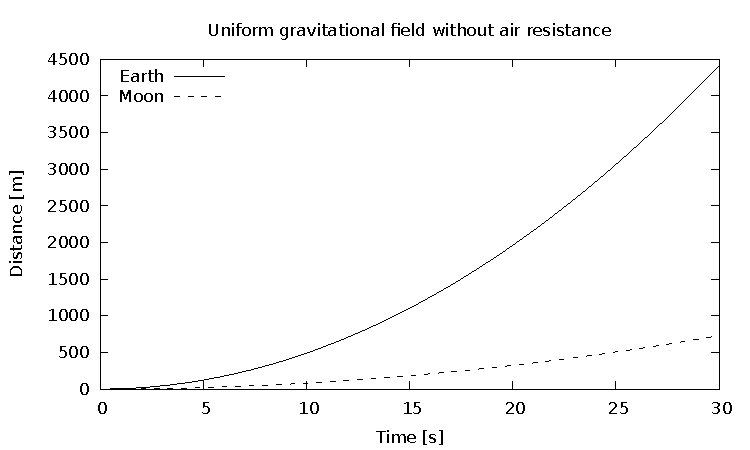
\includegraphics{gnuplot-bw}
% 	\caption{Černobílá varianta obrázku generovaného programem Gnuplot}\label{fig:gnuplot-bw}
% \end{figure}
% 
% \begin{figure}\centering
% 	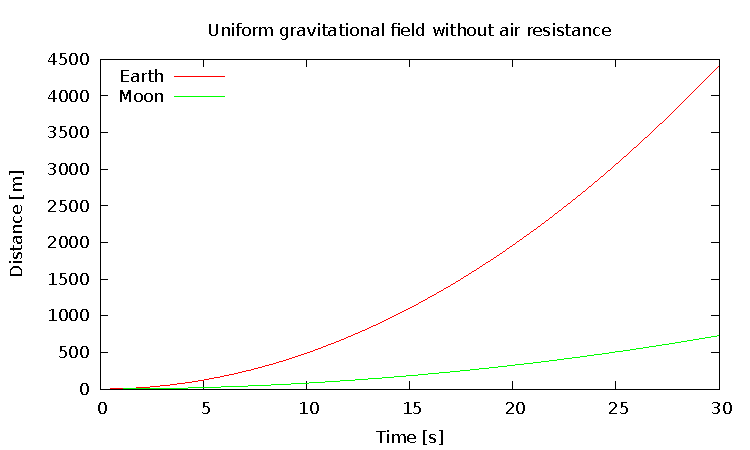
\includegraphics{gnuplot-col}
% 	\caption{Barevná varianta obrázku generovaného programem Gnuplot}\label{fig:gnuplot-col}
% \end{figure}
% 
% 
% \subsection{Tabulky}
% 
% Tabulky lze zadávat různě, např. v~prostředí \verb|tabular|, avšak pro jejich vkládání platí to samé, co pro obrázky -- použijte plovoucí prostředí, v~tomto případě \verb|table|. Například tabulka \ref{tab:matematika} byla vložena tímto způsobem.
% 
% \begin{table}\centering
% 	\caption[Příklad tabulky]{Zadávání matematiky}\label{tab:matematika}
% 	\begin{tabular}{|l|l|c|c|}\hline
% 		Typ		& Prostředí		& \LaTeX{}ovská zkratka	& \TeX{}ovská zkratka	\tabularnewline \hline \hline
% 		Text		& \verb|math|		& \verb|\(...\)|	& \verb|$...$|		\tabularnewline \hline
% 		Displayed	& \verb|displaymath|	& \verb|\[...\]|	& \verb|$$...$$|	\tabularnewline \hline
% 	\end{tabular}
% \end{table}
% 
% % % % % % % % % % % % % % % % % % % % % % % % % % % % 

\chapter{Obsah přiloženého CD}

%upravte podle skutecnosti

\begin{figure}
	\dirtree{%
		.1 readme.txt\DTcomment{stručný popis obsahu CD}.
		.1 exe\DTcomment{adresář se spustitelnou formou implementace}.
		.1 src.
		.2 impl\DTcomment{zdrojové kódy implementace}.
		.2 thesis\DTcomment{zdrojová forma práce ve formátu \LaTeX{}}.
		.1 text\DTcomment{text práce}.
		.2 thesis.pdf\DTcomment{text práce ve formátu PDF}.
		.2 thesis.ps\DTcomment{text práce ve formátu PS}.
	}
\end{figure}

\end{document}
